\chapter{Casi d'uso}
\label{UC}
In questa sezione sono elencati i casi d'uso del \textit{progetto$_{G}$}\glossario{MegAlexa}dedotti da un'attenta indagine ed analisi da parte dei membri del gruppo sugli attori principali del sistema, sulle loro caratteristiche e possibilità.
Ogni caso d'uso presenta i seguenti campi:
\begin{itemize}
	\item Codice identificativo;
	\item Titolo
	\item Attori primari;
	\item Attori secondari (se presenti);
	\item Descrizione;
	\item Precondizione;
	\item Postcondizione;
	\item Flusso principale degli eventi.
\end{itemize}
Se un caso d'uso risulta essere particolarmente complesso allora viene corredato da un diagramma dei casi d'uso in linguaggio UML.
\section{Codice identificativo CU}
Ogni caso d'uso deve avere la seguente nomenclatura:
\begin{center}
	\textbf{UC$\Bigl\{$XX$\Bigr\}$.$\Bigl\{$YY$\Bigr\}$}
\end{center}
dove:
\begin{itemize}
	\item \textbf{UC:} Use Case;
	\item \textbf{{XX}:} numero che identifica i casi d'uso;
	\item \textbf{{YY}:} numero progressivo che identifica i sottocasi, esso può, a sua volta, includere altri sottocasi.
\end{itemize}

\section{Attori dei casi d'uso}
\textbf{Attori primari}
\begin{itemize}
	\item \textbf{Utente non autenticato}: si riferisce all'utente del sistema che non ha ancora eseguito il login;
	\item \textbf{Utente autenticato}: si riferisce all'utente del sistema che ha effettuato il login ed è stato autenticato.
\end{itemize}
\textbf{Attori secondari}
\begin{itemize}
	\item \textbf{Amazon$_{G}$}.
\end{itemize}

\section{UC1: Scenario principale dell'utente non autenticato}
\label{UC1}
\begin{figure}[h]
	\centering
	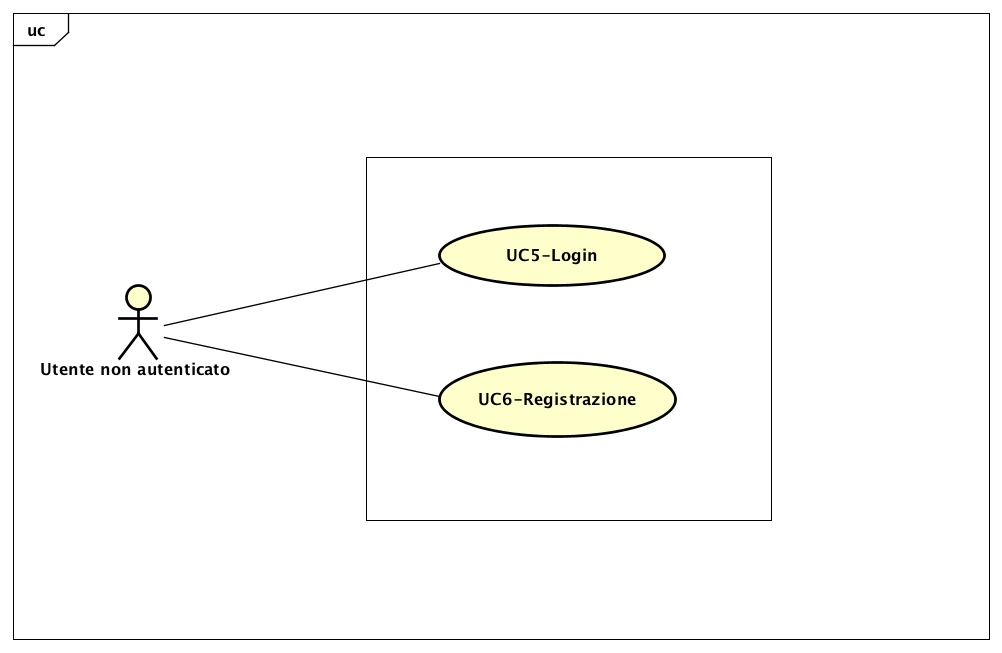
\includegraphics[scale=0.4]{Diagram/UC1.png}
	\caption{Scenario principale utente non autenticato}\label{}
\end{figure}
\begin{itemize}
	\item \textbf{Attori}: Amazon, Ut. non autenticato;
	\item \textbf{Descrizione}: Un utente non autenticato può registrarsi al nostro servizio se non ha ancora un account o effettuare il login, nel caso fosse già registrato
	\item \textbf{Precondizione}: L'applicazione è avviata e pronta all'uso
	\item \textbf{Postcondizione}: L'applicazione ha ricevuto tutte le informazioni dell'utente non autenticato sulle operazioni che vuole eseguire
	\item \textbf{Scenario principale}:
	\begin{enumerate} \item L'utente ha la possibilità di: Registrazione (UC1.1);  \item 
		L'utente ha la possibilità di: Login (UC1.2).\end{enumerate}
\end{itemize}

\section{UC1.1: Registrazione automatica}
\label{UC1.1}
\begin{itemize}
	\item \textbf{Attori}: Amazon, Ut. non autenticato;
	\item \textbf{Descrizione}: Per accedere al sistema è necessario possedere un account
	\item \textbf{Precondizione}: L'attore non possiede un account per accedere al sistema
	\item \textbf{Postcondizione}: E' stato creato un account per accedere al sistema
	\item \textbf{Scenario principale}:
	\begin{enumerate} \item L'utente preme il pulsante di login con Amazon;  \item  L'utente viene reinderizzato alla pagina web della registrazione con Amazon;  \item 
		L'utente completa la registrazione attraverso Amazon;  \item  L'utente ritorna nella pagina principale dell'applicazione e i suoi dati vengono salvati nel database.\end{enumerate}
\end{itemize}

\section{UC1.2: Login con Amazon}
\label{UC1.2}
\begin{itemize}
	\item \textbf{Attori}: Amazon, utente autenticato;
	\item \textbf{Descrizione}: Il sistema è avviato, ma è necessario effettuare il login per accedervi.
	\item \textbf{Precondizione}: Il sistema non permette l'accesso all'utente non autenticato.
	\item \textbf{Postcondizione}: Il sistema permette l'accesso all'utente che ora diventa un utente autenticato.
	\item \textbf{Scenario principale}:
	\begin{enumerate} \item L'utente preme il pulsante di login con Amazon;  \item  L'utente viene reinderizzato alla pagina web del login con Amazon;  \item 
		L'utente completa il login attraverso Amazon;  \item  L'utente ritorna nella pagina principale dell'applicazione.\end{enumerate}
	\item \textbf{Estensioni}:
	Login automatico (UC1.3).
\end{itemize}

\section{UC1.3: Login automatico}
\label{UC1.3}
\begin{itemize}
	\item \textbf{Attori}: Amazon, utente autenticato;
	\item \textbf{Descrizione}: Il sistema è avviato, ma è necessario effettuare il login per accedervi.
	\item \textbf{Precondizione}: Il sistema non permette l'accesso all'utente non autenticato.
	\item \textbf{Postcondizione}: Il sistema permette l'accesso all'utente che ora diventa un utente autenticato.
	\item \textbf{Scenario principale}:
	\begin{enumerate} \item Non c'erano scenari principali.\end{enumerate}
	\item \textbf{Scenari alternativi}:
	L'utente dopo aver inviato le proprie credenziali visualizza un messaggio d'errore (UC1.2.4).
\end{itemize}

\section{UC2: Scenario principale dell'utente autenticato}
\label{UC2}
\begin{figure} [h]
	\centering
	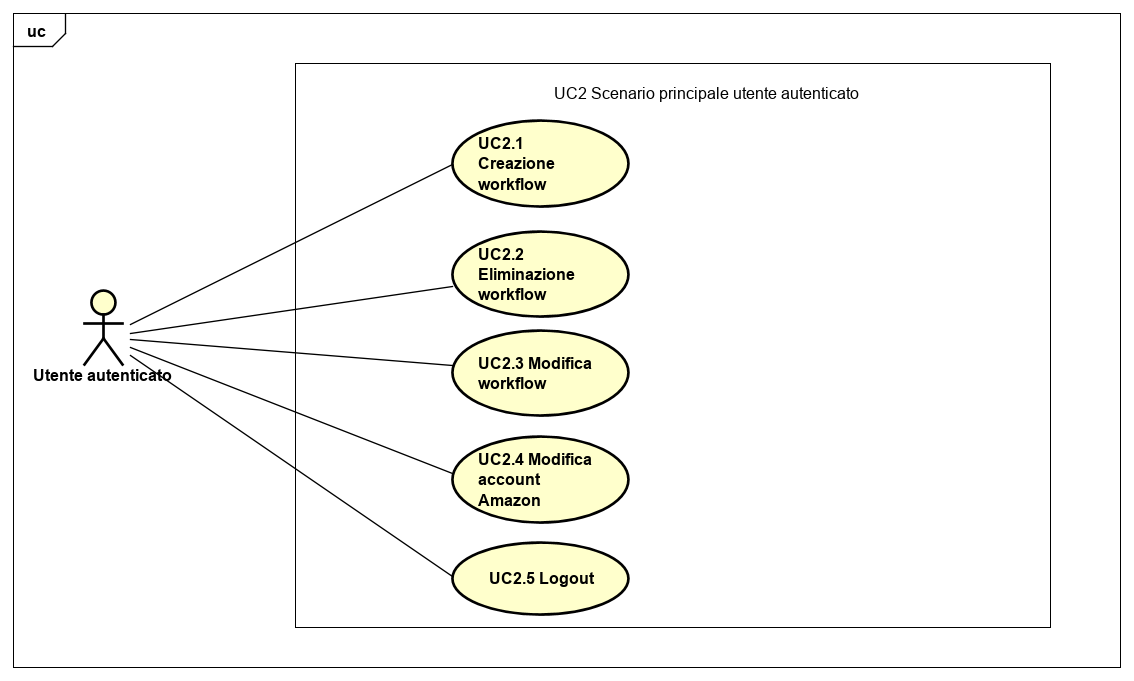
\includegraphics[scale=0.4]{./Diagram/UC2.png}
	\caption{Scenario principale dell'utente autenticato }\label{}
\end{figure}
\begin{itemize}
	\item \textbf{Attori}: Utente autenticato.
	\item \textbf{Descrizione}: L'attore può creare, modificare ed eliminare un workflow, modificare i propri dati personali ed eseguire il logout.
	\item \textbf{Precondizione}: Il sistema mostra la pagina principale per l'utente autenticato.
	\item \textbf{Postcondizione}: Il sistema ha ricevuto le informazioni riguardanti i comandi che l'utente vuole eseguire.
	\item \textbf{Scenario principale}:
	\begin{enumerate} \item L'utente può creare un workflow (UC2.1);  \item  L'utente può eliminare un workflow (UC2.2);  \item 
		L'utente può modificare un workflow (UC2.3);  \item  L'utente può modificare l'account Amazon (UC2.4);  \item 
		L'utente può effettuare il Logout (UC2.5).\end{enumerate}
\end{itemize}

\newpage
\section{UC2.1: Creazione workflow}
\label{UC2.1}

\begin{figure} [h]
	\centering
	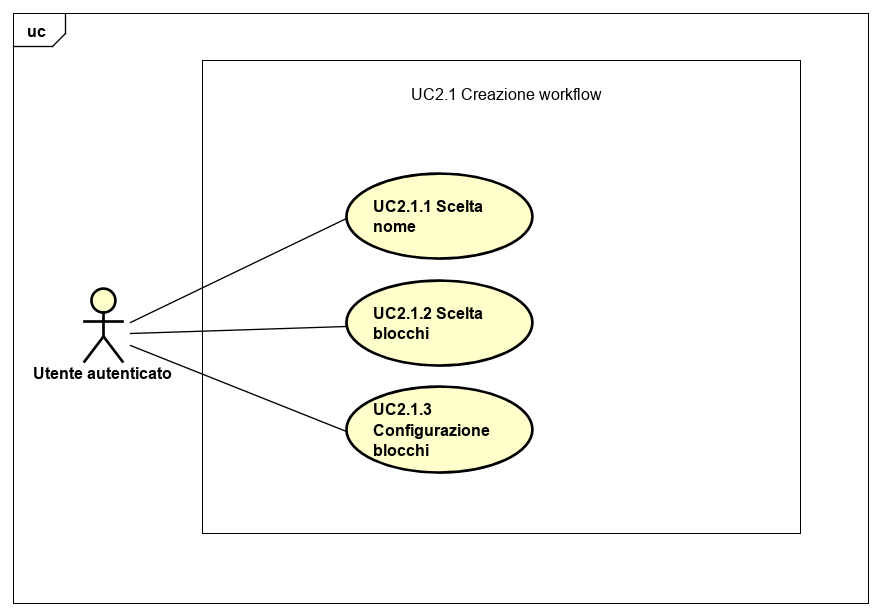
\includegraphics[scale=0.4]{./Diagram/UC2-1.png}
	\caption{Creazione workflow}\label{}
\end{figure}

\begin{itemize}
	\item \textbf{Attori}: Utente autenticato.
	\item \textbf{Descrizione}: L'attore può creare un workflow selezionando e configurando i blocchi disponibili.
	\item \textbf{Precondizione}: Il sistema mette a disposizione un form per la creazione di un workflow.
	\item \textbf{Postcondizione}: Il sistema contiene il workflow desiderato dall'attore.
	\item \textbf{Scenario principale}:
	\begin{enumerate} \item L'utente sceglie il nome del workflow (UC2.1.1);  \item  L'utente seleziona quali blocchi vuole aggiungere (UC2.1.2);  \item 
		L'utente configura i blocchi selezionati (UC2.1.3).\end{enumerate}
	\item \textbf{Scenari alternativi}:
	L'utente inserisce il nome del workflow non corretto
\end{itemize}

Essendo questo caso d'uso particolarmente articolato, riportiamo di seguito un diagramma di attività in modo da renderne più facile la comprensione.
\begin{figure} 
	\centering
	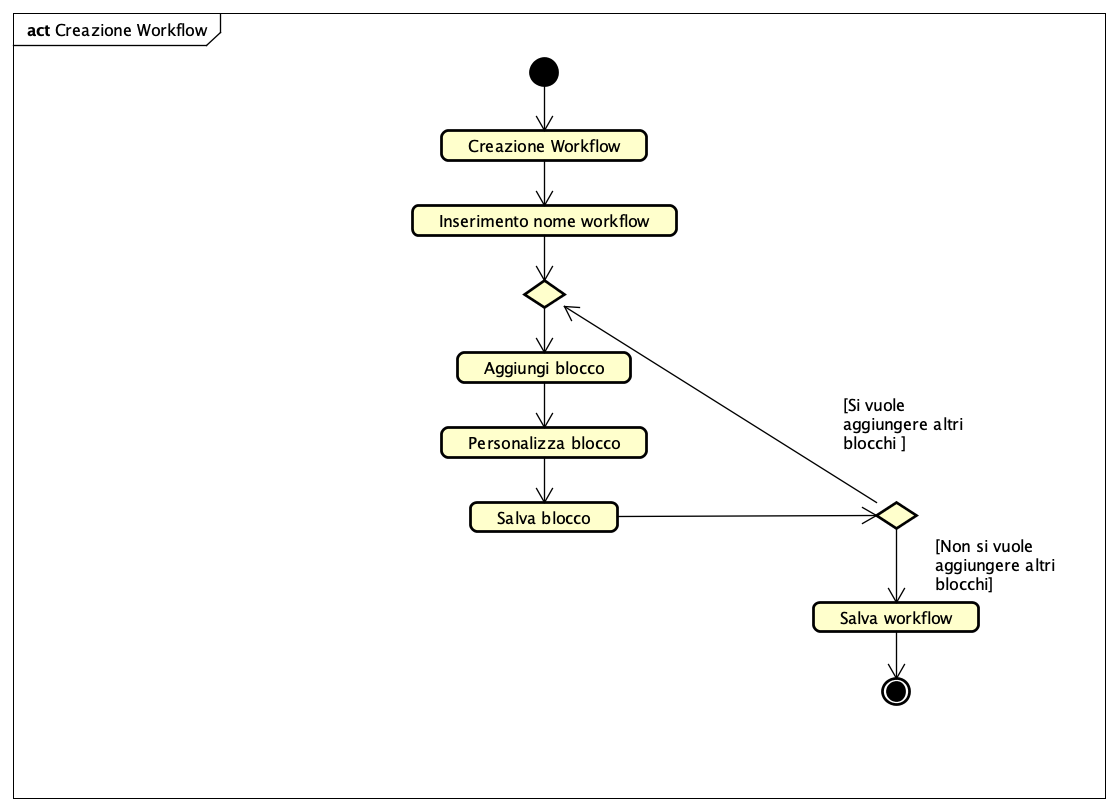
\includegraphics[scale=0.4]{./Diagram/CreazioneWorkflow.png}
	\caption{Diagramma di attività della creazione di un workflow}\label{}
\end{figure}



\section{UC2.1.1: Scelta nome}
\label{UC2.1.1}

\begin{itemize}
	\item \textbf{Attori}: Utente autenticato.
	\item \textbf{Descrizione}: L'attore inserisce il nome del workflow.
	\item \textbf{Precondizione}: Il sistema mette a disposizione un campo per l'inserimento del nome.
	\item \textbf{Postcondizione}: Il form di creazione del workflow contiene il nome del workflow.
	\item \textbf{Scenario principale}:
	\begin{enumerate} \item L'utente inserisce il nome del workflow.\end{enumerate}
\end{itemize}

\section{UC2.1.2: Scelta blocchi}
\label{UC2.1.2}
\begin{itemize}
	\item \textbf{Attori}: Utente autenticato.
	\item \textbf{Descrizione}: L'attore sceglie i blocchi che compongono il workflow. Può scegliere tra due categorie di blocchi: blocchi principali e blocchi di supporto.
	Blocchi principali: Twitter, Sveglia, Email, Telegram, Calendario, Youtube, Radio, Illuminazione, Spotify, Pianificazione, Notizie borsa e cryptovalute, Timer, Lista.
	Blocchi di supporto: Pin, Pianificazione, Filtro, Blocco di testo.
	\item \textbf{Precondizione}: Il sistema mette a disposizione un form per l'inserimento dei blocchi e una lista di blocchi disponibili.
	\item \textbf{Postcondizione}: Il workflow contiene i blocchi desiderati dall'utente.
	\item \textbf{Scenario principale}:
	\begin{enumerate} \item L'attore inserisce i blocchi nel form e li ordina come preferisce.\end{enumerate}
\end{itemize}

\section{UC2.1.2.1: Inserimento Pin}
\label{UC2.1.2.1}
\begin{itemize}
	\item \textbf{Attori}: Utente autenticato.
	\item \textbf{Descrizione}: L'attore può inserire il blocco "Pin" nel suo workflow. Questo blocco permette all'attore di proteggere il proprio workflow con un pin di 4 cifre. L'attore dovrà dire il pin ad Alexa prima di continuare con i blocchi che seguono.
	\item \textbf{Precondizione}: L'attore sta creando il workflow e il sistema gli permette di selezionare i blocchi
	\item \textbf{Postcondizione}: L'attore ha inserito il blocco Pin nel suo workflow
	\item \textbf{Scenario principale}:
	\begin{enumerate} \item L'attore seleziona il blocco Pin;  \item 
		L'attore inserisce il numero di 4 cifre richiesto dal sistema.\end{enumerate}
\end{itemize}

\section{UC2.1.2.2: Inserimento Pianificazione}
\label{UC2.1.2.2}
\begin{itemize}
	\item \textbf{Attori}: Utente autenticato.
	\item \textbf{Descrizione}: L'attore può inserire il blocco di supporto Pianificazione. Questo blocco indica quando far partire il prossimo blocco
	\item \textbf{Precondizione}: L'attore sta creando un workflow e il sistema permette di selezionare un blocco
	\item \textbf{Postcondizione}: L'attore ha inserito il blocco Pianificazione nel suo workflow
	\item \textbf{Scenario principale}:
	\begin{enumerate} \item L'attore include il blocco Pianificazione nel workflow.\end{enumerate}
\end{itemize}

\section{UC2.1.2.3: Inserimento Blocco di testo}
\label{UC2.1.2.3}
\begin{itemize}
	\item \textbf{Attori}: utente autenticato;
	\item \textbf{Descrizione}: L'attore può inserire un blocco di testo che verrà letto da Alexa.
	\item \textbf{Precondizione}: L'attore sta creando un workflow e il sistema permette di selezionare un blocco.
	\item \textbf{Postcondizione}: L'attore ha inserito il blocco di testo nel suo workflow
	\item \textbf{Scenario principale}:
	\begin{enumerate} \item L'attore seleziona il blocco;  \item  L'attore inserisce il testo.\end{enumerate}
\end{itemize}

\section{UC2.1.2.4: Inserimento Twitter}
\label{UC2.1.2.4}
\begin{itemize}
	\item \textbf{Attori}: utente autenticato;
	\item \textbf{Descrizione}: L'attore può inserire un blocco "Twitter" nel proprio workflow, che permette all'utente di pubblicare o rispondere ai tweet.
	\item \textbf{Precondizione}: L'attore sta creando un workflow e il sistema permette di selezionare un blocco
	\item \textbf{Postcondizione}: L'attore ha inserito le credenziali (del suo account Twitter) e configurato il blocco "Twitter".
	\item \textbf{Scenario principale}:
	\begin{enumerate} \item L'attore seleziona il blocco Twitter;  \item  L'attore inserisce le credenziali del proprio account;  \item  L'attore seleziona quali tweet vuole visualizzare (ordine cronologico, di importanza, account specifici).\end{enumerate}
\end{itemize}

\section{UC2.1.2.5: Inserimento Lista}
\label{UC2.1.2.5}
\begin{itemize}
	\item \textbf{Attori}: utente autenticato;
	\item \textbf{Descrizione}: L'attore può inserire un blocco "Lista" al suo workflow. Questo blocco permette all'attore di creare una lista, leggere e aggiungere elementi sia dall'applicazione che tramite Alexa
	\item \textbf{Precondizione}: L'attore sta creando un workflow e il sistema permette di selezionare un blocco
	\item \textbf{Postcondizione}: L'attore ha inserito il blocco "Lista" nel suo workflow.
	\item \textbf{Scenario principale}:
	\begin{enumerate} \item L'attore seleziona il blocco "Lista";  \item  L'attore popola la lista (opzionale).\end{enumerate}
\end{itemize}

\section{UC2.1.2.6: Inserimento Sveglia}
\label{UC2.1.2.6}
\begin{itemize}
	\item \textbf{Attori}: utente autenticato;
	\item \textbf{Descrizione}: L'attore può inserire un blocco "sveglia" nel suo workflow. La sveglia suona all'orario indicato dall'attore. L'attore può posporre o spegnere la sveglia (mente questa è attiva)
	\item \textbf{Precondizione}: L'attore sta creando un workflow e il sistema permette di selezionare un blocco.
	\item \textbf{Postcondizione}: L'attore ha inserito una sveglia nel suo workflow.
	\item \textbf{Scenario principale}:
	\begin{enumerate} \item L'attore seleziona il blocco "Sveglia";  \item  L'attore seleziona l'orario;  \item  L'attore seleziona quale tipo di suono riprodurre.\end{enumerate}
\end{itemize}

\section{UC2.1.2.7: Inserimento Mail}
\label{UC2.1.2.7}
\begin{itemize}
	\item \textbf{Attori}: Google, utente autenticato.
	\item \textbf{Descrizione}: L'attore può inserire un blocco "Mail" nel suo workflow. Questo blocco permette all'utente di leggere email tramite Alexa.
	\item \textbf{Precondizione}: L'attore sta creando un workflow e il sistema permette di selezionare un blocco.
	\item \textbf{Postcondizione}: L'attore ha inserito il blocco "Mail" e ha inserito le sue credenziali (della mail)
	\item \textbf{Scenario principale}:
	\begin{enumerate} \item L'attore seleziona il blocco Mail;  \item  L'attore inserisce le credenziali per accedere alla mail;  \item  L'attore seleziona quali tipi di email vuole leggere (tutte, più importanti, personalizzate).\end{enumerate}
\end{itemize}

\section{UC2.1.2.8: Inserimento Telegram}
\label{UC2.1.2.8}
\begin{itemize}
	\item \textbf{Attori}: Autent.Telegram, utente autenticato.
	\item \textbf{Descrizione}: L'attore può inserire un blocco "Telegram". Questo blocco permette la lettura e l'invio di messaggi vocali e testuali attraverso Alexa.
	\item \textbf{Precondizione}: L'attore sta creando un workflow e il sistema permette di selezionare un blocco.
	\item \textbf{Postcondizione}: L'attore ha inserito il blocco "Telegram" e le credenziali d'accesso nel suo workflow.
	\item \textbf{Scenario principale}:
	\begin{enumerate} \item L'attore seleziona il blocco "Telegram";  \item  L'attore inserisce le credenziali d'accesso.\end{enumerate}
\end{itemize}

\section{UC2.1.2.9: Inserimento Calendario}
\label{UC2.1.2.9}
\begin{itemize}
	\item \textbf{Attori}: Google, utente autenticato.
	\item \textbf{Descrizione}: L'attore può inserire il blocco "Calendario" e collegarlo al proprio calendario account Google. L'attore può inserire nuovi eventi tramite Alexa.
	\item \textbf{Precondizione}: L'attore sta creando un workflow e il sistema permette di selezionare un blocco.
	\item \textbf{Postcondizione}: L'attore ha inserito il blocco "Calendario" al proprio workflow.
	\item \textbf{Scenario principale}:
	\begin{enumerate} \item L'attore seleziona il blocco "Calendario";  \item  L'attore inserisce le proprie credenziali Google.\end{enumerate}
\end{itemize}

\section{UC2.1.2.10: Inserimento Youtube}
\label{UC2.1.2.10}
\begin{itemize}
	\item \textbf{Attori}: Google, utente autenticato.
	\item \textbf{Descrizione}: L'attore può inserire il blocco "Youtube" e collegarlo al proprio account Google.. Questo blocco permette all'attore di ascoltare musica attraverso youtube.
	\item \textbf{Precondizione}: L'attore sta creando un workflow e il sistema permette di selezionare un blocco.
	\item \textbf{Postcondizione}: L'attore ha inserito il blocco "Youtube" al proprio workflow.
	\item \textbf{Scenario principale}:
	\begin{enumerate} \item L'attore seleziona il blocco "Youtube";  \item  L'attore inserisce le proprie credenziali Google;  \item  L'attore inserisce gli url dei video che vuole riprodurre (solo audio).\end{enumerate}
	\item \textbf{Scenari alternativi}:
	Il video non esiste(UC2.1.2.10.1)
\end{itemize}

\section{UC2.1.2.10.1: Video Youtube inesistente}
\label{UC2.1.2.10.1}
\begin{itemize}
	\item \textbf{Attori}: Google, utente autenticato.
	\item \textbf{Descrizione}: L'attore ha inserito un url (di youtube) errato.
	\item \textbf{Precondizione}: L'attore ha provato a inserire un url (di youtube) che non esiste
	\item \textbf{Postcondizione}: Il sistema ha avvisato l'utente dell'inesistenza dell'url e gli permette di modificarlo oppure eliminarlo
	\item \textbf{Scenario principale}:
	\begin{enumerate} \item L'utente inserisce un url errato;  \item  Il sistema avvisa l'utente dell'inesistenza dell'url;  \item  L'utente modifica l'url o lo elimina.\end{enumerate}
\end{itemize}

\section{UC2.1.2.11: Inserimento timer}
\label{UC2.1.2.11}
\begin{itemize}
	\item \textbf{Attori}: Utente autenticato.
	\item \textbf{Descrizione}: L'attore può inserire un blocco "Timer" nel workflow. Questo blocco permette la riproduzione di un suono dopo un tempo specificato
	\item \textbf{Precondizione}: L'attore sta creando un workflow e il sistema permette di selezionare un blocco.
	\item \textbf{Postcondizione}: L'attore ha inserito il blocco "Timer".
	\item \textbf{Scenario principale}:
	\begin{enumerate} \item L'attore seleziona il blocco "Timer";  \item  L'attore inserisce il tempo che deve trascorrere prima;  \item  L'attore seleziona quale tipo di suono riprodurre.\end{enumerate}
\end{itemize}

\section{UC2.1.2.12: Inserimento Radio}
\label{UC2.1.2.12}
\begin{itemize}
	\item \textbf{Attori}: Utente autenticato.
	\item \textbf{Descrizione}: L'attore può inserire un modulo "Radio" nel workflow.
	\item \textbf{Precondizione}: L'attore sta creando un workflow e il sistema permette di selezionare un blocco.
	\item \textbf{Postcondizione}: L'attore ha inserito il blocco "Radio".
	\item \textbf{Scenario principale}:
	\begin{enumerate} \item L'attore seleziona il blocco "Radio";  \item  L'attore seleziona la stazione di default da riprodurre.\end{enumerate}
\end{itemize}

\section{UC2.1.2.13: Inserimento Illuminazione}
\label{UC2.1.2.13}
\begin{itemize}
	\item \textbf{Attori}: Utente autenticato.
	\item \textbf{Descrizione}: L'attore può accendere o spegnere le "lampadine intelligenti" collegate ad Alexa.
	\item \textbf{Precondizione}: L'attore sta creando un workflow e il sistema permette di selezionare un blocco.
	\item \textbf{Postcondizione}: L'attore ha inserito il blocco "Illuminazione".
	\item \textbf{Scenario principale}:
	\begin{enumerate} \item L'attore seleziona il blocco "Illuminazione";  \item  L'attore aggiunge le lampadine al blocco.\end{enumerate}
\end{itemize}

\section{UC2.1.2.14: Inserimento Spotify}
\label{UC2.1.2.14}
\begin{itemize}
	\item \textbf{Attori}: Spotify, utente autenticato.
	\item \textbf{Descrizione}: L'attore può inserire il blocco "Spotify" al workflow.
	\item \textbf{Precondizione}: L'attore sta creando un workflow e il sistema permette di selezionare un blocco.
	\item \textbf{Postcondizione}: L'attore ha inserito il blocco "Spotify"
	\item \textbf{Scenario principale}:
	\begin{enumerate} \item L'attore seleziona il blocco "Spotify";  \item  L'attore inserisce l proprie credenziali di Spotify;  \item  L'attore seleziona quale playlist riprodurre di default.\end{enumerate}
\end{itemize}

\section{UC2.1.2.15: Inserimento Borsa e Crypto}
\label{UC2.1.2.15}
\begin{itemize}
	\item \textbf{Attori}: Utente autenticato.
	\item \textbf{Descrizione}: L'attore può inserire il blocco "Borsa e Crypto". Questo blocco permette all'attore di conoscere i valori delle monete e cryptovalute. 
	\item \textbf{Precondizione}: L'attore sta creando un workflow e il sistema permette di selezionare un blocco.
	\item \textbf{Postcondizione}: L'attore ha inserito il blocco "Borsa e Crypto"
	\item \textbf{Scenario principale}:
	\begin{enumerate} \item L'attore seleziona il blocco "Borsa e Crypto";  \item  Il sistema fornisce una lista inerente di monete e criptovalute;  \item  L'attore seleziona le monete e criptovalute che vuole monitorare.\end{enumerate}
\end{itemize}

\section{UC2.1.2.16: Inserimento Feed RSS}
\label{UC2.1.2.16}
\begin{itemize}
	\item \textbf{Attori}: Utente autenticato.
	\item \textbf{Descrizione}: L'attore può inserire un feed RSS personalizzato.
	\item \textbf{Precondizione}: Il sistema mette a disposizione un form per l'inserimento dei blocchi e una lista di blocchi disponibili.
	\item \textbf{Postcondizione}: L'attore ha inserito il blocco di feed RSS.
	\item \textbf{Scenario principale}:
	\begin{enumerate} \item L'attore seleziona il blocco RSS;  \item  L'attore inserisce il link del feed RSS.\end{enumerate}
	\item \textbf{Scenari alternativi}:
	L'attore inserisce un url bagliato. (UC2.1.2.16.1)
\end{itemize}

\section{UC2.1.2.16.1: Feed RSS inesistente}
\label{UC2.1.2.16.1}
\begin{itemize}
	\item \textbf{Attori}: Utente autenticato;
	\item \textbf{Descrizione}: L'attore ha inserito un feed RSS non corretto
	\item \textbf{Precondizione}: L'attore ha inserito un feed RSS non corretto
	\item \textbf{Postcondizione}: L'attore ha inserito un feed RSS corretto, oppure ha annullato l'operazione.
	\item \textbf{Scenario principale}:
	\begin{enumerate} \item Il sistema chiede nuovamente il feed RSS oppure permette di annullare l'inserimento;  \item  L'attore inserisce un Feed RSS corretto oppure annulla l'operazione.\end{enumerate}
\end{itemize}

\section{UC2.1.2.17: Inserimento Filtro}
\label{UC2.1.2.17}
\begin{itemize}
	\item \textbf{Attori}: Utente autenticato.
	\item \textbf{Descrizione}: L'attore può inserire un blocco Filtro. Questo blocco va collegato ad un altro blocco, per filtrarne i risultati. 
	\item \textbf{Precondizione}: L'attore ha inserito un blocco compatibile con il Filtro e il sistema permette l'inserimento del prossimo blocco.
	\item \textbf{Postcondizione}: L'attore ha configurato il Filtro. 
	\item \textbf{Scenario principale}:
	\begin{enumerate} \item L'attore seleziona il Filtro;  \item  L'attore seleziona quanti record vuole filtrare.\end{enumerate}
\end{itemize}

\section{UC2.1.2.18: Inserimento Meteo}
\label{UC2.1.2.18}
\begin{itemize}
	\item \textbf{Attori}: Utente autenticato.
	\item \textbf{Descrizione}: L'attore può inserire il blocco Meteo. Questo blocco permette di conoscere il meteo nella città selezionata dall'attore.
	\item \textbf{Precondizione}: Il sistema mette a disposizione un form per l'inserimento dei blocchi e una lista di blocchi disponibili.	
	\item \textbf{Postcondizione}: L'attore ha inserito il blocco meteo e selezionato la città.
	\item \textbf{Scenario principale}:
	\begin{enumerate} \item L'attore seleziona il blocco Meteo;  \item  L'attore seleziona la città.\end{enumerate}
\end{itemize}

\section{UC2.1.2.19: Inserimento Amazon Music}
\label{UC2.1.2.19}
\begin{itemize}
	\item \textbf{Attori}: Amazon, utente autenticato.
	\item \textbf{Descrizione}: L'attore può inserire il blocco Amazon Music. Questo blocco permette di ascoltare la musica attraverso Amazon Music.
	\item \textbf{Precondizione}: L'attore sta creando un workflow e il sistema permette di selezionare un blocco.	
	\item \textbf{Postcondizione}: L'attore ha inserito il blocco workflow.
	\item \textbf{Scenario principale}:
	\begin{enumerate} \item L'attore seleziona il blocco Amazon Music;  \item  L'attore seleziona la playlist di default.\end{enumerate}
\end{itemize}

\section{UC2.2: Eliminazione workflow}
\label{UC2.2}
\begin{itemize}
	\item \textbf{Attori}: Utente autenticato.
	\item \textbf{Descrizione}: L'attore elimina un workflow.
	\item \textbf{Precondizione}: Il sistema mette a disposizione un comando per eliminare un workflow.
	\item \textbf{Postcondizione}: Il workflow che l'attore voleva eliminare è stato rimosso dal sistema.
	\item \textbf{Scenario principale}:
	\begin{enumerate} \item L'utente seleziona il comando per eliminare il workflow.\end{enumerate}
\end{itemize}

\section{UC2.3: Modifica workflow}
\label{UC2.3}
\begin{figure} [h]
	\centering
	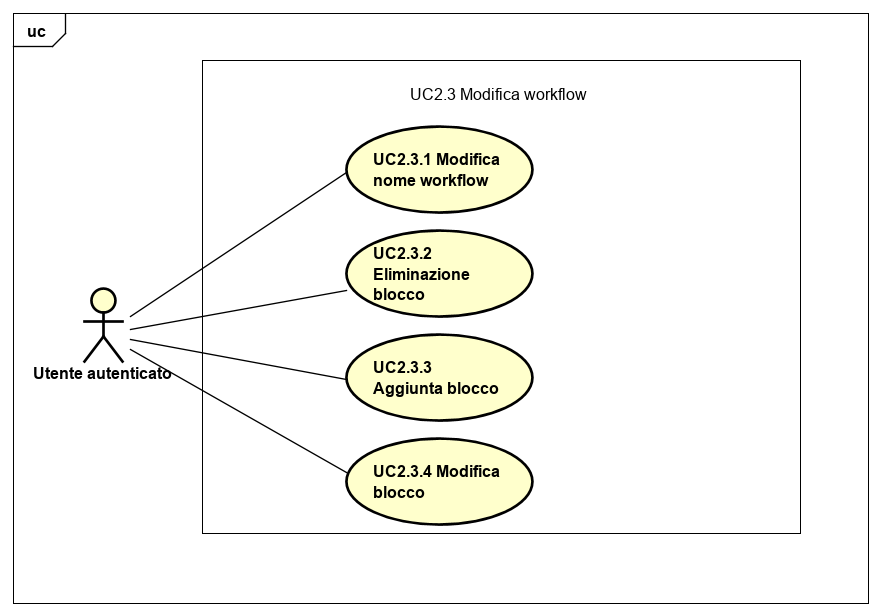
\includegraphics[scale=0.4]{./Diagram/UC2-3.png}
	\caption{Modifica workflow}\label{}
\end{figure}
\begin{itemize}
	\item \textbf{Attori}: Utente autenticato.
	\item \textbf{Descrizione}: L'attore modifica un workflow.
	\item \textbf{Precondizione}: Il sistema mette a disposizione un form per la modifica di un workflow.
	\item \textbf{Postcondizione}: Il workflow è stato modificato.
	\item \textbf{Scenario principale}:
	\begin{enumerate} \item L'attore può cambiare il nome del workflow (UC2.3.1);  \item  L'attore può eliminare un blocco dal workflow (UC2.3.2);  \item 
		L'attore può aggiungere un blocco nel workflow (UC2.3.3);  \item  L'attore può modificare la configurazione di un blocco presente nel workflow (UC2.3.4).\end{enumerate}
\end{itemize}

\section{UC2.3.1: Modifica nome workflow}
\label{UC2.3.1}
\begin{itemize}
	\item \textbf{Attori}: Utente autenticato.
	\item \textbf{Descrizione}: L'attore modifica il nome del workflow.
	\item \textbf{Precondizione}: Il sistema mette a disposizione un campo per l'inserimento del nuovo nome.
	\item \textbf{Postcondizione}: Il form di creazione del workflow contiene il nuovo nome del workflow.
	\item \textbf{Scenario principale}:
	\begin{enumerate} \item L'attore inserisce il nuovo nome del workflow.\end{enumerate}
\end{itemize}

\section{UC2.3.2: Eliminazione blocco}
\label{UC2.3.2}
\begin{itemize}
	\item \textbf{Attori}: Utente autenticato.
	\item \textbf{Descrizione}: L'attore rimuove il blocco che non desidera più nel workflow.
	\item \textbf{Precondizione}: Il sistema fornisce un comando per l'eliminazione del blocco.
	\item \textbf{Postcondizione}: Il workflow non contiene più il blocco indesiderato dall'attore.
	\item \textbf{Scenario principale}:
	\begin{enumerate} \item L'attore elimina il blocco.\end{enumerate}
\end{itemize}

\section{UC2.3.3: Aggiunta blocco}
\label{UC2.3.3}
\begin{itemize}
	\item \textbf{Attori}: Utente autenticato.
	\item \textbf{Descrizione}: L'attore aggiunge il nuovo blocco al workflow. La modalità di aggiunta blocchi è uguale a UC2.1.2.
	\item \textbf{Precondizione}: Il sistema mette a disposizione un form per l'aggiunta del blocco.
	\item \textbf{Postcondizione}: Il workflow contiene il nuovo blocco configurato.
	\item \textbf{Scenario principale}:
	\begin{enumerate} \item L'attore aggiunge il blocco;  \item  L'attore configura il nuovo blocco.\end{enumerate}
\end{itemize}

\section{UC2.3.4: Modifica blocco}
\label{UC2.3.4}
\begin{itemize}
	\item \textbf{Attori}: Utente autenticato.
	\item \textbf{Descrizione}: L'attore modifica la configurazione del blocco che compone il workflow.
	\item \textbf{Precondizione}: Il sistema mette a disposizione un form per la modifica dei blocchi.
	\item \textbf{Postcondizione}: Il blocco desiderato dall'attore è stato riconfigurato.
	\item \textbf{Scenario principale}:
	\begin{enumerate} \item L'attore modifica la configurazione del blocco.\end{enumerate}
\end{itemize}

\section{UC2.4: Modifica account Amazon}
\label{UC2.4}
\begin{itemize}
	\item \textbf{Attori}:Utente autenticato.
	\item \textbf{Descrizione}: L'attore cambia il proprio account Amazon.
	\item \textbf{Precondizione}: Il sistema mette a disposizione un form per la modifica dell'account Amazon.
	\item \textbf{Postcondizione}: Il sistema è collegato al nuovo account Amazon.
	\item \textbf{Scenario principale}:
	\begin{enumerate} \item L'attore, attraverso il form di Amazon, sceglie il nuovo account.\end{enumerate}
	\item \textbf{Estensioni}:
	Visualizzazione dell'errore di cambio Account (UC2.4.1).
\end{itemize}

\section{UC2.4.1: Errore di cambio account Amazon}
\label{UC2.4.1}
\begin{itemize}
	\item \textbf{Attori}: Utente autenticato.
	\item \textbf{Descrizione}: L'attore ha inserito dei dati non corretti e non riesce a collegarsi al nuovo account Amazon.
	\item \textbf{Precondizione}: Il sistema non riesce a collegarsi all'account Amazon.
	\item \textbf{Postcondizione}: Il sistema è correttamente collegato a un account Amazon.
	\item \textbf{Scenario principale}:
	\begin{enumerate} \item L'attore può inserire nuovamente i dati nel form di Amazon;  \item  L'attore può tornare al vecchio account Amazon.\end{enumerate}
\end{itemize}

\section{UC2.5: Logout}
\label{UC2.5}
\begin{itemize}
	\item \textbf{Attori}:Utente autenticato.
	\item \textbf{Descrizione}: L'attore effettua il logout dall'applicazione.
	\item \textbf{Precondizione}: Il sistema fornisce un metodo per permettere all'utente di disconnettersi dal sistema.
	\item \textbf{Postcondizione}: Il sistema non riconosce più l'utente.
	\item \textbf{Scenario principale}:
	\begin{enumerate} \item L'attore si disconnette dal sistema.\end{enumerate}
\end{itemize}

